%% ------------------------------------------------------------------------- %%
\chapter{Introdução}
\label{cap:introducao}


Com o advento dos repositórios de código-fonte aberto e das comunidades abertas de perguntas e respostas de programação, a busca por código-fonte tornou-se uma atividade cotidiana no processo de desenvolvimento de software \citep{towards-summarizing-source-code-search:marin:2020}. De acordo com \cite{what-developers-search-for-on-the-web:xia:2017}, os programadores gastam em média 15\% do seu tempo efetivo de trabalho realizando buscas, por exemplo, acerca do uso de bibliotecas de programação, significados de mensagens de erro ou buscando como um trecho de código funciona. Segundo \cite{sadowski-how-developers-search-for-code-case-study:2015}, os desenvolvedores do Google realizam em média 12 buscas por dia, clicando em torno de 2 a 3 resultados por busca. De acordo com os pesquisadores, o propósito da maior parte das buscas é encontrar exemplos de trechos de código-fonte. A capacidade de recuperar trechos de código-fonte relevantes torna-se uma importante ferramenta para a produtividade do desenvolvedor. 

Atualmente, a maioria dos desenvolvedores recorrem a ferramentas de busca como o Google, que utilizam estratégias de indexação e ranqueamento de páginas que não são otimizadas para código-fonte. Nesse caso, os buscadores não conseguem extrair a semântica por trás do código-fonte, a não ser que o código esteja acompanhado de um texto explicativo. Segundo \cite{masudur-developers-use-google-code-retrieval:2018}, os desenvolvedores demoram mais, visitam mais páginas web e alteram com mais frequência uma consulta para encontrar um resultado relevante para sua pesquisa relacionada a código-fonte quando comparada a uma busca não relacionada a código.

\begin{figure}[H]
\centering
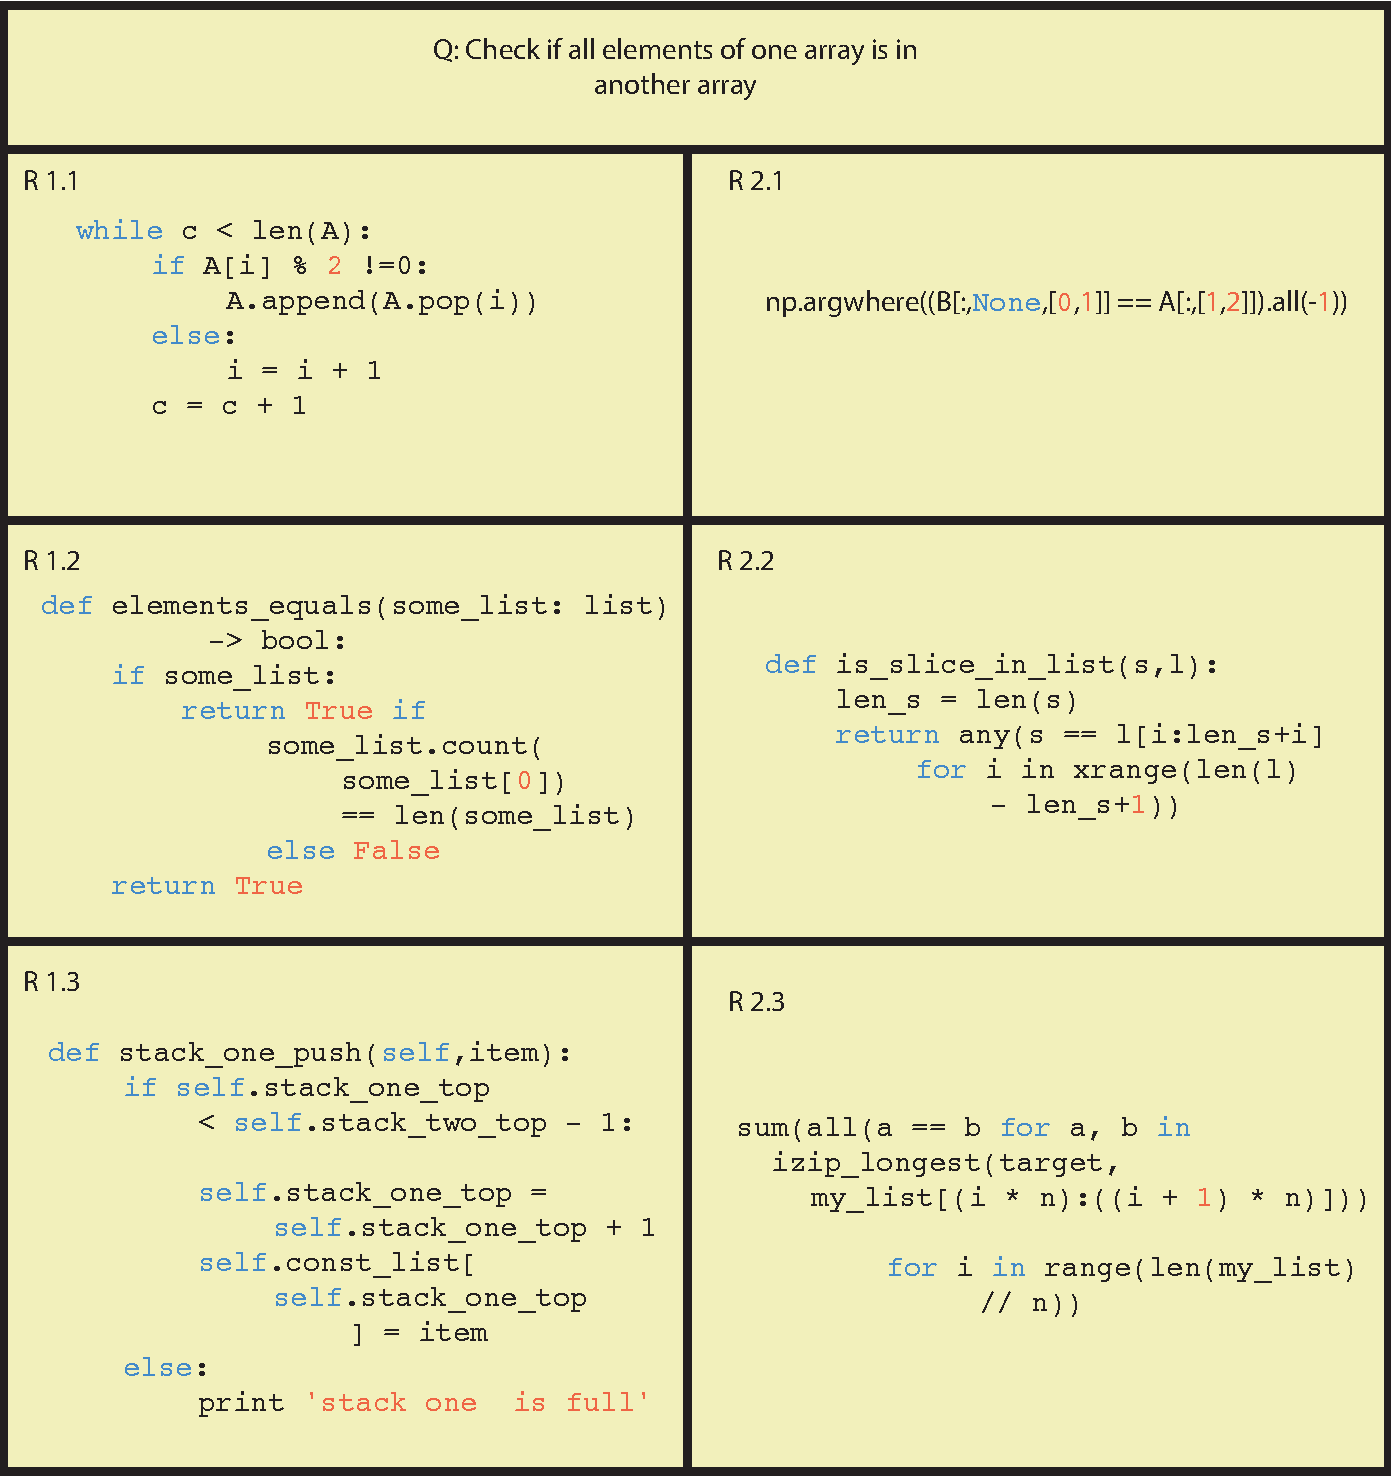
\includegraphics[width=0.7\textwidth]{figuras/cap-introducao/concrete_examples.pdf}
\caption[Exemplo]{Exemplo comparativo de respostas dadas pelo Github e o nosso modelo à pergunta \emph{Q}, que verifica se um vetor é subconjunto de outro vetor. As respostas exibidas como resultado pela busca do Github não conseguem responder à pergunta \textbf{Q} (respostas \textbf{R 1.x}). A primeira resposta exibida (R 1.1) retorna um vetor com números pares seguido de números ímpares, enquanto a segunda (R 2.2) exibe uma função que verifica se os elementos de uma lista são iguais. O nosso modelo apresenta a resposta correta (R 2.2) e, além disso, exibe uma outra solução que verifica subconjuntos em matrizes (R 2.1). A consulta no Github foi realizada dia 07 de Dezembro de 2020 com filtros para exibir apenas códigos-fontes em Python.} 
\label{fig:concrete-example}
\end{figure}

A busca por trechos de código tem sido um desafio. Atualmente, o site do GitHub, que hospeda milhares de projetos de código-aberto, não possui um mecanismo de pesquisa que
seja capaz de recuperar um trecho de código-fonte relevante a partir dos termos utilizados no campo de sua busca (ver Figura~\ref{fig:concrete-example}). Pesquisadores do GitHub tentaram criar uma busca semântica associando milhares de trechos de código a comentários \gls{docstring} extraídos de repositórios do próprio \Gls{github}. Porém, os resultados não foram satisfatórios, pois a busca somente retornava resultados relevantes quando o usuário utilizava palavras-chaves similares às palavras presentes nos comentários \gls{docstring} \citep{husain-github-semantic-search-code-2019}. 

Pesquisadores do Facebook \citep{cambronero-deep-learning-code-search:2019} também abordarem este problema e constataram que comentários \gls{docstring} não conseguem extrair a semântica do código-fonte de forma a atender às intenções do usuário em uma busca. Esses pesquisadores verificaram que as intenções dos usuários foram melhor expressas através de questões extraídas de comunidades abertas de perguntas e respostas, como o \gls{sof}. No caso do \Gls{sof}, os usuários expressam suas perguntas em linguagem natural e outros usuários podem responder com trechos de código-fonte. O usuário que fez a pergunta pode indicar qual é a resposta correta, enquanto outros usuários podem votar na resposta mais relevante ou eleger uma resposta incorreta. Essas ações coletivas feitas pelos usuários ajudam na curadoria e organização da informação, facilitando a busca por informações relevantes \citep{Wang-quora:2013, cambronero-deep-learning-code-search:2019}. 


Diversos trabalhos foram feitos com o intuito de propor uma maneira de recuperar trechos de código-fonte. Os primeiros trabalhos utilizavam ferramentas baseadas em regras lógico-dedutivas e extração manual de caractéristicas do código-fonte \citep{Allamanis:2018:SML}. Com o sucesso das redes neurais artificiais, devido à disponibilidade de recurso computacional e do advento da era do \textit{Big Data}, a maior parte dos trabalhos passaram a empregar técnicas baseadas em aprendizagem de máquina utilizando redes neurais artificiais \citep{Gu-deep-code-search:2018, yao-2018, iyer-etal-2016-summarizing, Allamanis-bimodal-source-code-natural-language:2015, Chen-bi-variational-autoencoder:2018, Sachdev-neural-code-search:2018, cambronero-deep-learning-code-search:2019}. \cite{cambronero-deep-learning-code-search:2019} cunharam o termo \textit{neural code search}, i.e., busca de código-fonte através do uso de redes neurais artificiais.

A maior parte dos trabalhos aplicou redes neurais artificiais para sumarizar e recuperar trechos de código-fonte \citep{iyer-etal-2016-summarizing, Allamanis-bimodal-source-code-natural-language:2015, Chen-bi-variational-autoencoder:2018}. Sumarização e recuperação automática de código-fonte são duas tarefas distintas, cada uma com suas peculiaridades, desafios e métricas de avaliação de desempenho \citep{allahyari-text-summarization-2017}. Segundo \cite{Allamanis-bimodal-source-code-natural-language:2015}, as redes neurais apresentaram uma maior dificuldade na tarefa de recuperação de trechos de código-fonte quando comparada à sumarização. De acordo com os pesquisadores, as redes neurais tiveram dificuldades em discriminar os trechos de código-fonte relevantes, pois a diferença entre os termos presentes nos trechos de código relevantes e não relevantes é bem sutil.

O nosso trabalho propõe uma nova abordagem de arquitetura de redes neurais artificiais para a tarefa de recuperação de trechos de código-fonte. Diferente do trabalho de \cite{Gu-deep-code-search:2018} que propôs uma arquitetura com redes neurais recorrentes e do trabalho de \cite{cambronero-deep-learning-code-search:2019}, que utilizou redes neurais com mecanismo de atenção, a nossa abordagem é baseada em redes neurais convolucionais, que apresentaram um bom desempenho em tarefas de seleção de resposta em \acrshort{nlp} \citep{feng-2015, tan-lstm-qa, wen-joint-modeling-question-answer-2019}. Os trabalhos de \cite{Gu-deep-code-search:2018} e \cite{cambronero-deep-learning-code-search:2019} associaram trechos de código a comentários \gls{docstring}, enquanto o nosso trabalho utilizou os dados disponibilizados por \cite{yao-2018}, que são compostos de questões e trechos de código-fonte extraídas do \Gls{sof}.

%% ------------------------------------------------------------------------- %%
\section{Objetivos}
\label{sec:objetivo}

O principal objetivo deste trabalho é propor uma abordagem  para a recuperação de trecho de código-fonte. Avaliamos a eficácia das redes neurais convolucionais na tarefa de discriminar os trechos de código-fonte relevantes dos não-relevantes para uma questão. Para isto, comparamos a nossa arquitetura com outras duas arquiteturas de referência: uma arquitetura de rede neural mais simples que serve como base de comparação e a arquitetura proposta por \cite{cambronero-deep-learning-code-search:2019}, que utiliza o mecanismo de atenção e é o estado da arte atualmente. Os experimentos foram realizados utilizando uma base de dados disponibilizada por \cite{yao-2018}, composta por questões e trechos de código-fonte em Python e SQL coletadas do site StackOverflow. No nosso trabalho, utilizamos apenas as questões e trechos de código-fonte em Python.

%% ------------------------------------------------------------------------- %%
\section{Contribuições}
\label{sec:contribucoes}

Dentre as contribuições deste trabalho estão:

\begin{itemize}
\item Proposta de uma nova abordagem utilizando redes neurais convolucionais para a tarefa de recuperação de trechos de código-fonte;
\item Avaliação da eficácia do desempenho da nova arquitetura com relação a outras duas arquiteturas;
\item Disponibilização do código-fonte, desde o pré-processamento até a avaliação final, em um repositório público.
\end{itemize}

\subsection{Outras contribuições}

Durante o programa do mestrado, publicamos dois artigos apresentando os resultados deste trabalho:

\begin{itemize}
    \item Marcelo de Rezende Martins and Marco Aurélio Gerosa. 2019. Um estudo preliminar sobre o uso de uma arquitetura deep learning para seleção de respostas no problema de recuperação de código-fonte. In Anais do VII Workshop on Software Visualization, Evolution and Maintenance (VEM), (pp. 94-101). Porto Alegre: SBC. DOI: \url{https://doi.org/10.5753/vem.2019.7589}.
    \item Marcelo de Rezende Martins and Marco Aurélio Gerosa. 2020. CoNCRA: A Convolutional Neural Network Code Retrieval Approach. In 34th Brazilian Symposium on Software Engineering (SBES ’20), October 21 - 23, 2020, Natal, Brazil. ACM, New York, NY, USA, 6 pages. \url{https://doi.org/10.1145/3422392.3422462}
\end{itemize}


%% ------------------------------------------------------------------------- %%
\section{Organização do Trabalho}
\label{sec:organizacao_trabalho}

No Capítulo~\ref{cap:fundamentacao-teorica}, apresentamos os conceitos e trabalhos relacionados à recuperação de trecho de código-fonte. No Capítulo~\ref{cap:abordagem}, apresentamos a nossa abordagem para o item de pesquisa proposto. No Capítulo~\ref{cap:experimento}, detalhamos o conjunto de dados e os procedimentos utilizados para treinamento e avaliação das redes neurais artificiais. Os resultados dos experimentos foram exibidos e discutidos no Capítulo~\ref{cap:resultados}. Expomos as nossas conclusões e observações acerca de trabalhos futuros no Capítulo~\ref{cap:conclusoes}.